\begin{figure*}[tp]
\centering
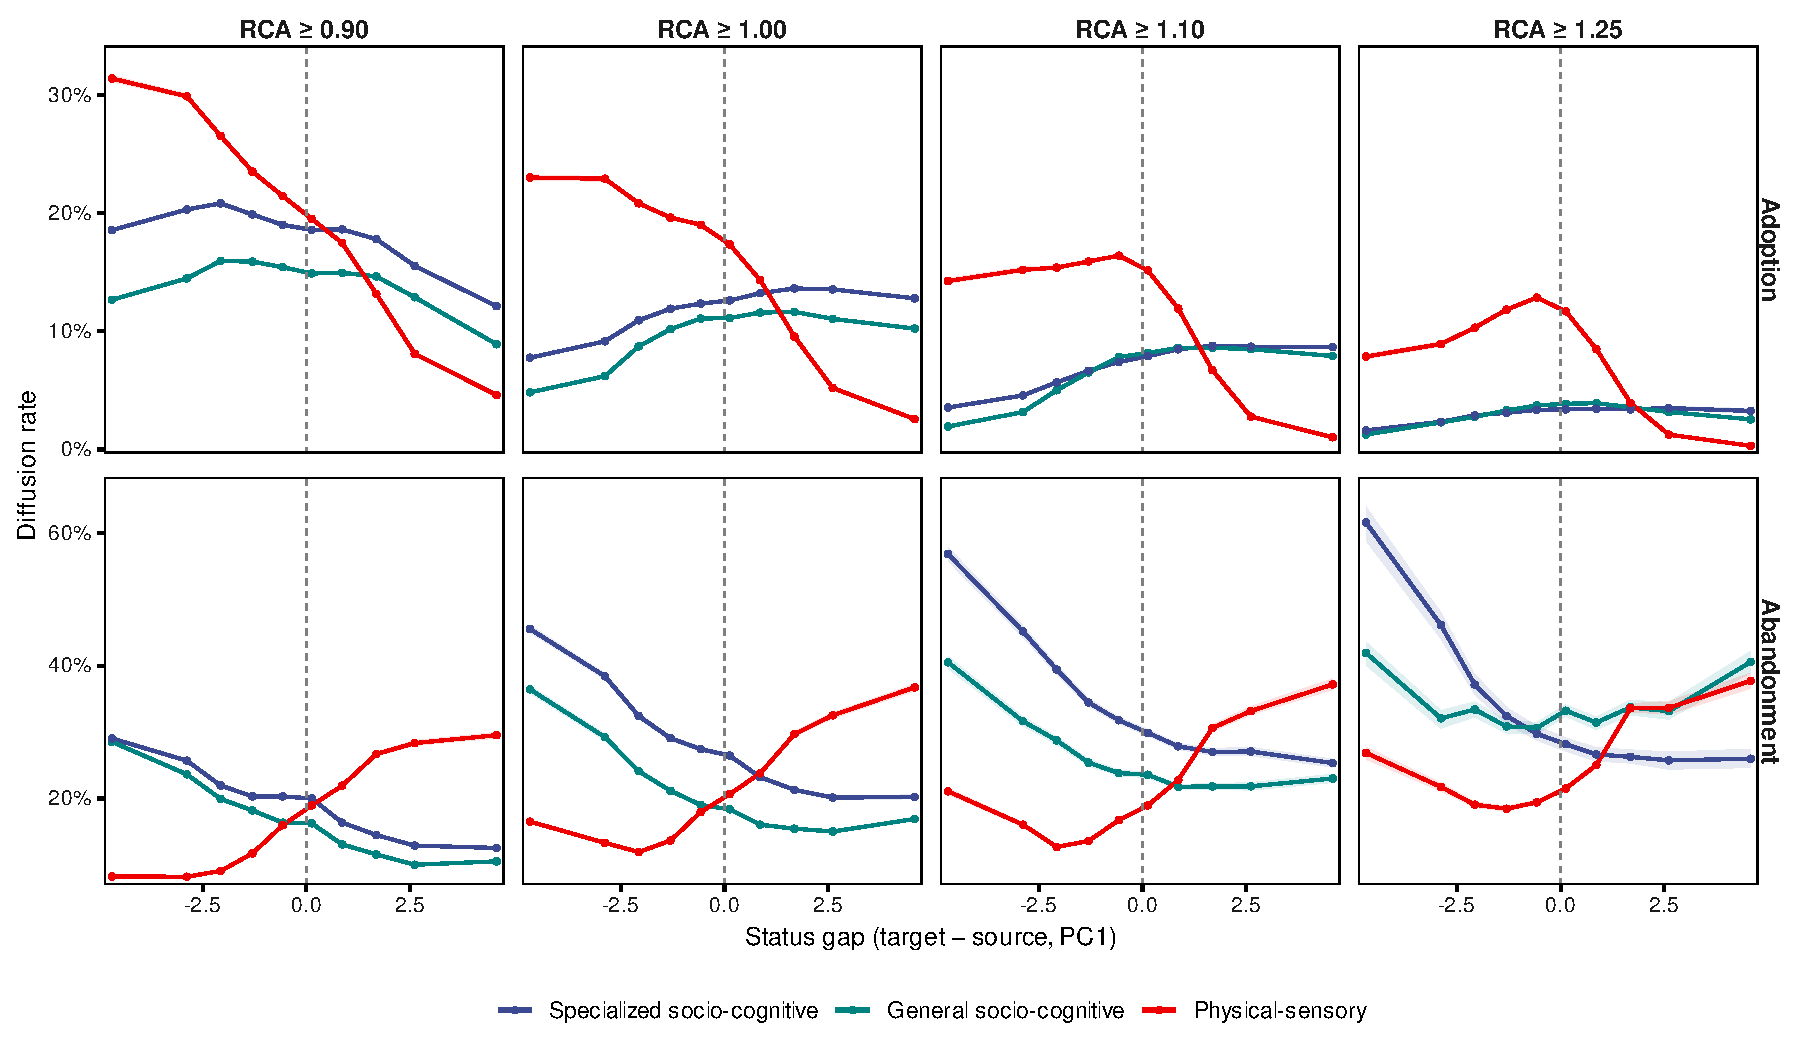
\includegraphics[width=0.95\textwidth]{figures/fig_S1_rca_threshold.pdf}
\caption{\textbf{Directional diffusion gradients are insensitive to the RCA specialization threshold.} Each panel plots the observed diffusion rate as a function of the signed status gap (target $-$ source, PC1) for one of four specialization thresholds ($\mathrm{RCA} \geq 0.90$, $1.00$, $1.10$, $1.25$; rows) and two flows (Adoption, Abandonment; columns). Colors identify the three skill types. Ribbons are 95\% bootstrap confidence intervals ($B = 500$). The directional asymmetry---socio-cognitive rates rising with the gap, sensory-physical rates falling---is present at every threshold in both flows. O*NET 2015--2024.}
\label{fig:SI_rca}
\end{figure*}
